\documentclass[12pt]{article}
\usepackage[utf8]{inputenc}
\usepackage[russian]{babel} %comment it for english!
\usepackage{amsfonts,longtable,amssymb,amsmath,array}
\usepackage{graphicx}
\usepackage{euscript}
\usepackage{graphicx}
\usepackage{xcolor}
\usepackage{hyperref}
\graphicspath{ {images/} }
\definecolor{linkcolor}{HTML}{799B03} % цвет ссылок
\definecolor{urlcolor}{HTML}{799B03} % цвет гиперссылок 
\hypersetup{pdfstartview=FitH,  linkcolor=linkcolor,urlcolor=urlcolor, colorlinks=true}
\newtheorem{vkTheorem}{Theorem}[section]
\newtheorem{vkLemma}[vkTheorem]{Lemma}
\newenvironment{vkProof}%
   {\par\noindent{\bf Proof.\par\nopagebreak}}%
   {\hfill$\scriptstyle\blacksquare$\par\medskip}
%\textwidth=450pt%%
%\textheight=650pt
%\oddsidemargin=0pt
%\hoffset=0pt
%\voffset=0pt
%\topmargin=0pt
%\headheight=0pt
%\headsep=0pt
\newcommand{\suml}[0]{\sum\limits}
\begin{document}


\section*{Арзуманян Виталий, CS, 2 курс}

\subsection*{Общее описание}
В рамках выполнения домашнего задания был реализован набор скриптов по скачиванию simple.wikipedia.org, построению статистики и обработке, а так же по подсчету и отображению нескольких характеристик. Исходные файлы приложены. 

\subsection*{Компоненты}
Решение состоит из нескольких частей. 

\subsubsection*{Загрузка}
Функция downloadSimpleWiki() обходит заданный сайт и скачивает html-файлы страничек в папку /docs. Фильтруются "бесполезные" ссылки по правилам из функции isWikiArticle(). На вход не принимает ничего, на выходе имеем: папка /docs с html-файлами скачанных страничек и файлом urls, содержащим ссылку, id, и отметку об успешности загрузки, а так же файл linkpathes.tsv, содержащий записи вида id страницы, ссылка для списка возможных переходов между страницами. Работает долго, основная часть - задержка 1с. между просмотрами страниц, все действия помимо задержки не превышают 0.2с. Время работы не сохранилось, около 2 суток. Скачано 163705 документов.

Интересный график количества документов в очереди - до некоторого момента примерно экспоненциально растет, затем почти линейно падает:
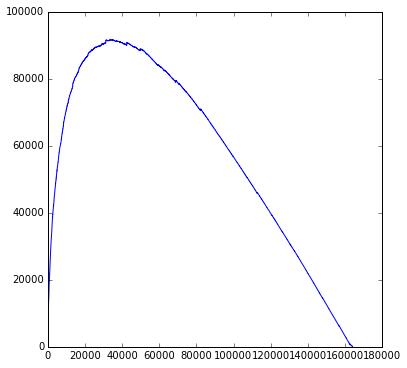
\includegraphics[scale=0.7]{downloadingspeed.png}

\subsubsection*{Предобработка}
Функция process() работает со скачанными html-файлами, фалойм urls, и файлом linkpathes.tsv. На выходе имеем папку /text с выделенными текстами документов (отсеяны те, которые скачаны, но не являются статьями - по доп. условиям из функции linkIsBad(), т.е. те, который были недоотсеяны на первом этапе + вспомогательные странички /Category:), файл urls.dat в корневом каталоге, содержащий список id и ссылок на скачанные документы, разделенные пробелами и файл graph.dat, содержащий список направленных ребер, состоящих из id ссылок, а так же файл sizes.dat с размерами скачанных документов для последующего отображения. В текст преобразовано 136814 документов.

\subsubsection*{Обработка графа}
Функция graphprocess() работает со списком направленных ребер из файла graph.dat. Граф строится только на скачанном подмножетсве страниц (именно скачанном, не преобразованном в текст). Характеристики построенного графа: $M=7492648$ ребер, $N=163705$ вершин. Делается несколько вещей: сохраняет список ребер с исходящими степенями и список ребер с входящими степенями для последующего отображения (indegrees.tsv и outdegrees.tsv), алгоритмом Дейкстры (выбран оптимизированный алгоритм Дийкстры как ассимптотически наилучший на графе с такими характеристиками - время работы оценивается как $O(N\log N + M\log N)$) находятся кратчайшие пути до вершин из исходной (с номером 1) и сохраняются в файл patheslengths.tsv, так же простейшей вариацией алгоритма PageRank с начальными весами $1/n$ считаются ранги страниц и сохраняются в файл ranks.tsv. Для PageRank было взято значение $\varepsilon=10^{-7}$ для оценки разности изменения l2-нормы массива рангов, алгоритм сошелся за 307 шагов.

\subsubsection*{Подсчет слов}
Функция words() обходит все скачанные документы (лежащие в папке /text) и на выходе составляет список слов с количеством их появлений в коллекции, сохраняется в wordfreq.tsv

\subsubsection*{Отображение}
Отображение всего, что нужно для задания, делается в iPython notebook по предподготовленным файлам. Не включено в основной скрипт, т.к. не является содержательным. ipynb-файл так же приложен.

\subsection*{Характеристики}
\subsubsection*{Гистограмма распределения размеров документов}
Гистограмма с логарифмической осью y. Видно, что размер почти экспоненциально пропорционал количеству до 500Kb, дальше идут только выбросы. Основное количество документов сосредоточено до 100Kb

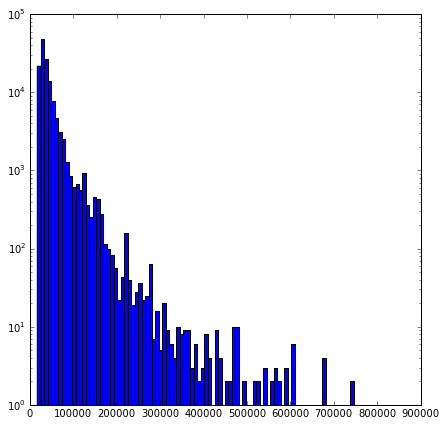
\includegraphics[scale=0.7]{1.png}

\subsubsection*{Гистограмма распределения степеней вершин}
Гистограмма с логарифмическими осями. Исходящие - красные, входящие - зеленые. Распределения входящих и исходящих степеней близки приблизительно до степени $10^3$ и зависимость логарифмических осей почти линейна. Затем в до степени порядка $10^4$ идет более резкий спад для входящих степеней, для исходящих же на порядке $10^3$ спад почти до нуля. Есть выросы вплоть до максимальной степени 163075 для входящих степеней, а для исходящих максимум 2046.

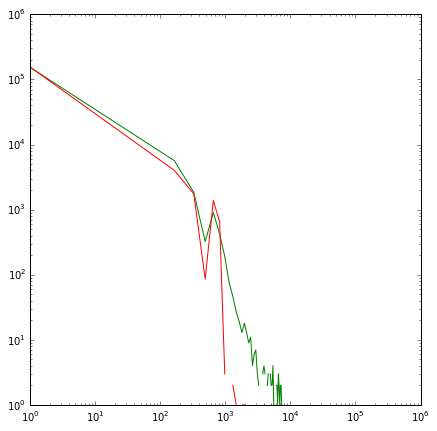
\includegraphics[scale=0.7]{22.png}

\subsubsection*{Гистограмма распределения расстояний от главной страницы}
Интересная гистограмма распределение расстояний. Граф, очевидно, связный - т.к. сам процесс скачивания был обходом из одной точки, следовательно, скачанная часть полного графа связна. Максимальное расстояние 7, минимальное расстояние 0 только до одной вершины. Ниже приведены гистограммы в логарифмических и линейных осях. Видно, что распределение сдвинуто в сторону расстояний 3 и 4.

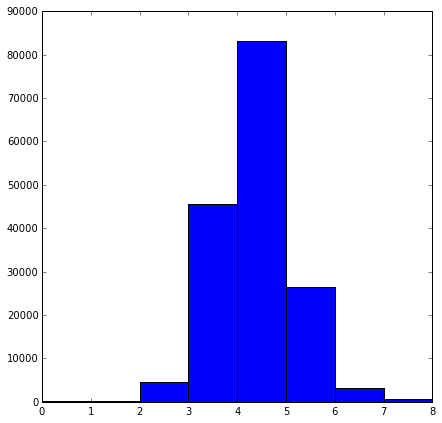
\includegraphics[scale=0.7]{3.png}
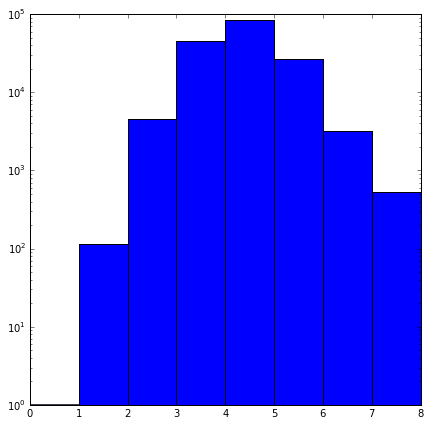
\includegraphics[scale=0.7]{4.png}

\subsubsection*{Гистограмма распределения частот слов}
Гистограмма распределения частот слов в логарифимических осях. Почти равномерная линейная зависимость логарифмических осей от порядка $10^6$ слов для близких к нулю частот до $10^2$ для частот $10^5$. Дальше спад до нуля, менее гладкий.

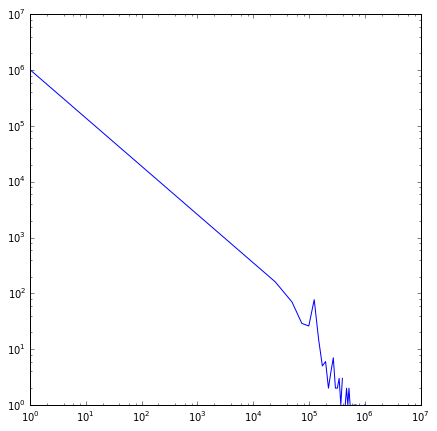
\includegraphics[scale=0.7]{5.png}


\subsubsection*{TOP20 страниц по PageRank}
С большим отрывом лидирует главная страница, т.к. на нее ссылаются все. Дальше - страны, религии, общие понятия, несколько категорий. Не стал отсеивать не-статьи при построении PageRak, т.к. при отсеивании граф теряет связность - хотелось бы построить по полному. \\
0.0389 \url{http://simple.wikipedia.org/wiki/Main_Page}\\
0.0068 \url{http://simple.wikipedia.org/wiki/Multimedia}\\
0.0045 \url{http://simple.wikipedia.org/wiki/Category:Stubs}\\
0.0028 \url{http://simple.wikipedia.org/wiki/United_States}\\
0.0024 \url{http://simple.wikipedia.org/wiki/Definition}\\
0.0019 \url{http://simple.wikipedia.org/wiki/Category:Basic_English_850_words}\\
0.0018 \url{http://simple.wikipedia.org/wiki/English_language}\\
0.0017 \url{http://simple.wikipedia.org/wiki/Category:Technology_stubs}\\
0.0015 \url{http://simple.wikipedia.org/wiki/Country}\\
0.0015 \url{http://simple.wikipedia.org/wiki/International_Standard_Book_Number}\\
0.0015 \url{http://simple.wikipedia.org/wiki/Category:Geography_stubs}\\
0.0013 \url{http://simple.wikipedia.org/wiki/Category:Disambiguation}\\
0.0013 \url{http://simple.wikipedia.org/wiki/United_Kingdom}\\
0.0013 \url{http://simple.wikipedia.org/wiki/Government}\\
0.0013 \url{http://simple.wikipedia.org/wiki/Mathematics}\\
0.0012 \url{http://simple.wikipedia.org/wiki/France}\\
0.0012 \url{http://simple.wikipedia.org/wiki/Category:Biology_stubs}\\
0.0011 \url{http://simple.wikipedia.org/wiki/Language}\\
0.0011 \url{http://simple.wikipedia.org/wiki/Europe}\\
0.0011 \url{http://simple.wikipedia.org/wiki/Christianity}\\

Если посмотреть на рейтинг только статей, будет похожая картина.\\
0.0389 \url{http://simple.wikipedia.org/wiki/Main_Page}\\
0.0068 \url{http://simple.wikipedia.org/wiki/Multimedia}\\
0.0028 \url{http://simple.wikipedia.org/wiki/United_States}\\
0.0024 \url{http://simple.wikipedia.org/wiki/Definition}\\
0.0018 \url{http://simple.wikipedia.org/wiki/English_language}\\
0.0015 \url{http://simple.wikipedia.org/wiki/Country}\\
0.0015 \url{http://simple.wikipedia.org/wiki/International_Standard_Book_Number}\\
0.0013 \url{http://simple.wikipedia.org/wiki/United_Kingdom}\\
0.0013 \url{http://simple.wikipedia.org/wiki/Government}\\
0.0013 \url{http://simple.wikipedia.org/wiki/Mathematics}\\
0.0012 \url{http://simple.wikipedia.org/wiki/France}\\
0.0011 \url{http://simple.wikipedia.org/wiki/Language}\\
0.0011 \url{http://simple.wikipedia.org/wiki/Europe}\\
0.0011 \url{http://simple.wikipedia.org/wiki/Christianity}\\
0.0011 \url{http://simple.wikipedia.org/wiki/Animal}\\
0.001 \url{http://simple.wikipedia.org/wiki/Audience}\\
0.001 \url{http://simple.wikipedia.org/wiki/Law}\\
0.001 \url{http://simple.wikipedia.org/wiki/Information}\\
0.001 \url{http://simple.wikipedia.org/wiki/Wiktionary}\\

\begin{flushright}
$\Box$
\end{flushright}

\end{document} 
